\documentclass{article}
\newcommand{\rg}{\text{rg}}
% file's preambule
%%%%%%%%%%%%%%%%%%%



% connect packages
\usepackage[T2A]{fontenc}
\usepackage[utf8]{inputenc}
\usepackage[english]{babel}
\usepackage{hyperref}     % ТАК_НУЖНО
\hypersetup{unicode=true} % ТАК_НУЖНО
\usepackage{amsmath}
\usepackage{amssymb,textcomp, esvect,esint}
\usepackage{amsfonts}
\usepackage{amsthm}
\usepackage{graphicx}
\usepackage{indentfirst}
\usepackage{xcolor}
% \usepackage{enumitem} %--- ломал нумерацию!?

\usepackage{graphicx}
\usepackage{booktabs}
\usepackage{caption}
\usepackage{listings}
\usepackage{tikz}
\usepackage{xcolor}



\usepackage{media9}
\usepackage{animate}
\usepackage{threeparttable}
\usepackage{pifont}


\usepackage{import}
\usepackage{xifthen}
\usepackage{pdfpages}
\usepackage{transparent}

\usepackage[skip=1pt]{caption}

% create environment

\newtheorem{to_thr}{Thr}[section]
\newtheorem{to_suj}[to_thr]{Suj}
\newtheorem{to_lem}[to_thr]{Lem}
\newtheorem{to_com}[to_thr]{Com}
\newtheorem{to_con}[to_thr]{Con}
\theoremstyle{definition}
\newtheorem{to_def}[to_thr]{Def}


\newenvironment{itemize*}
{
    \begin{itemize}
        \setlength{\itemsep}{1pt}
        \setlength{\parskip}{1pt}}
    {\end{itemize}
}

\newenvironment{enumerate*}
{
    \begin{enumerate}
        \setlength{\itemsep}{1pt}
        \setlength{\parskip}{1pt}}
    {\end{enumerate}
}

\newenvironment{description*}
{
    \begin{description}
        \setlength{\itemsep}{1pt}
        \setlength{\parskip}{1pt}}
    {\end{description}
}


\newenvironment{hw1}
{
    \phantom{42}

    \noindent
    \textbf{Домашнее задание:} \hrulefill
    % \vspace{-2mm}
    % \begin{enumerate*}

}
{
    % \end{enumerate*}
    \vspace{2mm}
    \hrule

    \phantom{42}
}


\newenvironment{hw2}
{
    \phantom{42}

    \noindent
    \textbf{Домашнее задание:} \hrulefill
    \vspace{-2mm}
    \begin{enumerate*}

}
{
    \end{enumerate*}
    \hrule

    \phantom{42}
}

% document palette
\definecolor{ugreen}{RGB}{0, 100, 0}
\definecolor{ured}{RGB}{220, 0, 0}
\definecolor{ugray}{RGB}{90, 90, 90}

% \newcommand{\red}[1]{\textcolor{ured}{#1}}
% \newcommand{\green}[1]{\textcolor{ugreen}{#1}}


\definecolor{grey}{HTML}{666666}
\definecolor{linkcolor}{HTML}{0000CC}
\definecolor{urlcolor}{HTML}{006600}
\hypersetup{
    pdfstartview=FitH,  
    linkcolor=linkcolor,
    urlcolor=urlcolor, 
    colorlinks=true,
    citecolor=blue}

% add (renew) commands
% add (renew) commands

\renewcommand{\Im}{\mathop{\mathrm{Im}}\nolimits}
\renewcommand{\Re}{\mathop{\mathrm{Re}}\nolimits}

\renewcommand{\d}{\, d}
\renewcommand{\leq}{\leqslant}
\renewcommand{\geq}{\geqslant}
\renewcommand{\l}{\left}
\renewcommand{\r}{\right}

\newcommand{\vc}[1]{\mbox{\boldmath $#1$}}
\newcommand{\T}{^{\text{T}}}


\newcommand{\diag}{\mathop{\mathrm{diag}}\nolimits}
\newcommand{\cl}{\mathop{\mathrm{cl}}\nolimits}
\newcommand{\grad}{\mathop{\mathrm{grad}}\nolimits}
\renewcommand{\div}{\mathop{\mathrm{div}}\nolimits}
\newcommand{\rot}{\mathop{\mathrm{rot}}\nolimits}
\newcommand{\Ker}{\mathop{\mathrm{Ker}}\nolimits}
\newcommand{\Spec}{\mathop{\mathrm{Spec}}\nolimits}
\newcommand{\sign}{\mathop{\mathrm{sign}}\nolimits}
\newcommand{\tr}{\mathop{\mathrm{tr}}\nolimits}
\newcommand{\rg}{\mathop{\mathrm{rg}}\nolimits}


\newcommand{\DS}{\mathcal D\left(\mathbb{R}\right)}
\newcommand{\QED}{\textnormal{Q. E. D.}}
\newcommand{\dseq}{\overset{\mathcal D'}{=}}
\newcommand{\dto}{\overset{\mathcal D'}{\to}}


\newcommand{\const}{\text{const}}
\newcommand{\xmark}{\ding{55}}


\newenvironment{uproof}{
% \begin{comment}
\par \color{ugray}
\begin{proof}[$\triangle$]
}{
\end{proof} \par
% \end{comment}
}


\newcommand{\bhat}{\overset{\text{\scalebox{0.8}[0.5]{\rotatebox[origin=c]{180}{$\wedge$}}}}}

\newcommand{\cf}[1]{\text{\raisebox{1.5pt}{$\scalebox{1.3}{$\chi$}$}}_{#1}}

\newcommand{\supp}{\mathop{\mathrm{supp}}\nolimits}
\newcommand{\si}{\mathop{\mathrm{Si}}\nolimits}

\newcommand{\rr}{\rightrightarrows}

% \newcommand{\sbsnum}[2]{
%     \setcounter{subsection}{\the\numexpr #1 - 1 \relax}
%     \subsection{#2}
% }

% Секции и сабсекции
% \definecolor{darkblue}{HTML}{000099}
% \newcommand{\sbs}[1]{\subsection{\textcolor{darkblue}{#1}}}
% \renewcommand{\sec}[1]{\section{\textcolor{darkblue}{#1}}}
\newcommand{\sbs}[2]{
\setcounter{subsection}{\numexpr #1 - 1 \relax}
    \textcolor{ugreen}{
        \subsection{#2}
        }
}



% add page header
% add page header

\pagestyle{fancy}
\fancyhf{}
\fancyhead[RE,LO]{\textsc{Ф\raisebox{-1.5pt}{и}з\TeX}}
\fancyhead[LE,RO]{Ж\raisebox{-1.5pt}{и}К}
\fancyhead[CO,CE]{\leftmark}
\fancyfoot[LE,RO]{\textcolor{grey}{\texttt{\thepage}}}



% matrixes shortcuts 
% \newcommand{\dmat}[4]{
  \ifthenelse{
    \equal{#1}{3}
  }{
\begin{pmatrix}
    #2 & 0 & 0 \\
    0 & #3 & 0 \\
    0 & 0 & #4 \\
\end{pmatrix}
  }{
  \ifthenelse{
      \equal{#1}{2}
    }{
  \begin{pmatrix}
      #2 & 0 \\
      0 & #3 \\
  \end{pmatrix}
    }{
      \text{\textcolor{red}{error}}
    }
  }
}

\newcommand{\skmat}[4]{
  \ifthenelse{
    \equal{#1}{3}
  }{
\begin{pmatrix}
    0 & -#4 & #3 \\
    #4 & 0 & -#2 \\
    -#3 & #2 & 0 \\
\end{pmatrix}
  }{
  \ifthenelse{
      \equal{#1}{2}
    }{
  \begin{pmatrix}
      0 & #2 \\
      -#2 & 0 \\
  \end{pmatrix}
    }{
      \text{\textcolor{red}{error}}
    }
  }
}

% additional symbols and commands


\DeclareRobustCommand{\tmpsim}{ %%%%%%%%%%%%%% ~ < %%%%%%%%%%%%%%%%%%%
  \mathbin{\text{
      \raisebox{-1pt}{
            \hspace{-4.5pt} \rotatebox{-26}{\scalebox{0.8}[0.7]{$\sim$}}
        }
  }}
}
\def\lesim{{
    \setbox0\hbox{$\ <\ $}
    \rlap{\hbox to \wd0{\hss$\tmpsim$\hss}}\box0
}}
%%%%%%%%%%%%%%%%%%%%%%%%%%%%%%%%%%%%%%%%%%%%%%%%%%%%%%%%%%%%%%%%%%%%%%


\def\letuscom{%%%%%%%%%%%%%%%%%%%%%% ПУСТЬ %%%%%%%%%%%%%%%%%%%%%%%%%%
\mathord{\setbox0=\hbox{$\exists$}%
     \hbox{\kern 0.125\wd0%
           \vbox to \ht0{%
              \hrule width 0.75\wd0%
              \vfill%
              \hrule width 0.75\wd0}%
           \vrule height \ht0%
           \kern 0.125\wd0}%
   }%
}
\newcommand{\letus}{\raisebox{-1.2pt}{$\letuscom$}}
%%%%%%%%%%%%%%%%%%%%%%%%%%%%%%%%%%%%%%%%%%%%%%%%%%%%%%%%%%%%%%%%%%%%%%


\usepackage{arydshln} %%%%%%%%%%%%%%% ЛИНИИ В МАТРИЧКЕ %%%%%%%%%%%%%%%
\makeatletter
  \renewcommand*\env@matrix[1][*\c@MaxMatrixCols c]{%
    \hskip -\arraycolsep
    \let\@ifnextchar\new@ifnextchar
  \array{#1}}
\makeatother
%%%%%%%%%%%%%%%%%%%%%%%%%%%%%%%%%%%%%%%%%%%%%%%%%%%%%%%%%%%%%%%%%%%%%%


\makeatletter %%%%%%%%%%%%%%% КРУЖОЧЕК %%%%%%%%%%%%%%%%%%%%%%%%%%%%%%%
\newcommand*{\encircled}[1]{\relax\ifmmode\mathpalette
\@encircled@math{#1}\else\@encircled{#1}\fi}
\newcommand*{\@encircled@math}[2]{\@encircled{$\m@th#1#2$}}
\newcommand*{\@encircled}[1]{%
  \tikz[baseline,anchor=base]{\node[draw,circle,outer sep=0pt,
                                        inner sep=.2ex] {#1};}}
\makeatother
%%%%%%%%%%%%%%%%%%%%%%%%%%%%%%%%%%%%%%%%%%%%%%%%%%%%%%%%%%%%%%%%%%%%%%











\begin{document}


\setlength{\abovedisplayskip}{3pt}
\setlength{\abovedisplayshortskip}{3pt}
\setlength{\belowdisplayskip}{3pt}
\setlength{\belowdisplayshortskip}{3pt}

% \numberwithin{equation}{section}

\begin{center}
    \LARGE \textsc{Задание по курсу <<Дифференциальные уравнения II>>}
\end{center}

\hrule

\phantom{42}

\begin{flushright}
    \begin{tabular}{rr}
    % written by:
        \textbf{Автор}: 
        & Шишкин П.Е. \\ 
        &\\
    % date:
        \textbf{От}: &
        \textit{\today}\\
    \end{tabular}
\end{flushright}

\thispagestyle{empty}
\tableofcontents 
\newpage


\section{От авторов}
\subsection{Шрифт для личных сообщений}
\textcolor[rgb]{0.480469, 0.566406, 0.480469}{\textit{Меня попросили писать текст не имеющий отношения к решению как-то выделенно, поэтому отныне текст, который я пишу просто от души и сердца, будет написан курсивным шрифтом цвета лягушки в обмороке (я серьёзно, такой цвет есть)}}
\subsection{Благодарности}                                            
\textcolor[rgb]{0.480469,0.566406,0.480469}{\textit{Я благодарен *список людей* за *причины* FIXME}}
\subsection{Заходите в гости}
 \textcolor[rgb]{0.480469,0.566406,0.480469}{\textit{Заходите в гости, всегда всем рад :)}}                                                                                              

\section{I. Первые интегралы и их использование для решений автономных систем}
\subsection{C. \S14: 12}
Исследовать при всех значениях вещественного параметра $a$ поведение фазовых траекторий на всей фазовой плоскости для системы:
\begin{equation}
    \begin{cases}
       \dot{x} = y + ax(x^2 + y^2 - 2)\\
        \dot{y} = - x + ay(x^2 + y^2 - 2)\\
    \end{cases}
\end{equation}
Уравнение выглядит, как что-то в полярных координатам. Чтож, перейдём к ним 
\begin{align*}
x = r \sin{(\varphi)}&&\dot{x} = r \cos {(\varphi)} \dot{\varphi} + \dot{r} \sin {(\varphi )} \\ 
y = r \cos{(\varphi)}&&\dot{y} = -r \sin {(\varphi)} \dot{\varphi} + \dot{r} \cos {(\varphi )} \\ 
\end{align*}
Откуда:
\begin{equation*}
    \begin{cases}
       r \cos {(\varphi)} \dot{\varphi} + \dot{r} \sin {(\varphi )} = r \cos{(\varphi)} + ar \sin{(\varphi)}(r^2 - 2)\\  
      -r \sin {(\varphi)} \dot{\varphi} + \dot{r} \cos {(\varphi )} = -r \sin{(\varphi)} + ar \cos{(\varphi)}(r^2 - 2)\\
    \end{cases}
\end{equation*}
Откуда можно получить 
\begin{equation*}
\begin{cases}
    \dot{r}=ra(r^2-2)\\
    \dot{\varphi}=1\\
        \end{cases}
\end{equation*}
Здесь уже очевидны 3 случая: 1)$a>0$, 2)$a<0$ 3) $a=0$. 1) неустойчивый предельный цикл радиуса $\sqrt 2$ 2) устойчивый 
предельный цикл радиуса $\sqrt 2$  3) центр. Разница при различных знакоопределённых параметрах будет в скорости "навивания" на предельный цикл, но характер движения будет схожий.\\
 Кстати, $\dot{\varphi}=1$ - это первый интеграл. В целом мы сказали при каких параметрах, что но можно это всё безобразие построить \ref{fig:14.12}.\textcolor[rgb]{0.480469,0.566406,0.480469}{\textit{Чтобы было максимально красиво, построим фазовую диаграмму для $r$ график в декартовых координатах и зависимость угла от радиуса. Кстати такая фигня с производной фи получилась из-за неклассической замены икса с синусом. Т.е. немного контринтуитивно что $\varphi =1$ это цикл по часовой стрелке, но и замена $x=\sin{(\varphi)}$ это что-то безумное (я просто хотел кушать а не думать)}}
\begin{figure}[h!]
\center{\includegraphics[width=1\linewidth]{14.12.png}}
\caption{Фазовые диаграммы 14.12 в различных координатах для различных параметров}
\label{fig:14.12}
\end{figure}                                                                 
\subsection{Ф.: 1149}
Решить систему уравнений:
\begin{equation}\label{f1149}
    \begin{cases}
       \dot{x}=y-x\\
       \dot{y}=x+y+z\\
       \dot{x}=x-y\\
    \end{cases}
\end{equation}
Довольно очевидно, что выделить 2 каких-то уравнения без третьей переменной тут не выйдет  \textcolor[rgb]{0.480469,0.566406,0.480469}{(\textit{ну или я слишком слаб и не могу этого сделать)}} поэтому воспользуемся правилом пропорции (чёрной магией):
\begin{equation*}
A/B=C/D=E/F=k;\forall \alpha, \beta,\gamma \in \mathbb{R}, \alpha^2+\beta^2+\gamma^2 \neq 0 \rightarrow \frac{\alpha A + \beta C + \gamma E}{\alpha B + \beta D + \gamma F}=k                                                 
\end{equation*}
Тогда можно записать учитывая $k=dt$:
\begin{equation*}
    \frac{\alpha dx + \beta dy + \gamma dz}{\alpha (y-x) + \beta (x+y+z) + \gamma (x-y)}=dt                                       
\end{equation*}      \
Возьмём $\alpha=1, \beta=0, \gamma=1$ тогда знаменатель обнулится, а значит и числитель должен быть ноль  \textcolor[rgb]{0.480469,0.566406,0.480469}{\textit{(на самом деле можно было бы сформулировать этот шаг гораздо проще, просто вычитая первое и третье уравнения друг из друга, но 1) правило пропорции весьма полезная штуковина в этих задачах, так что чего бы не сформулировать его, 2) обожаю делить на 0 эхэхэхэхэ}}\\
Итак, мы получаем что: $dx+dz=0$ а значит мы нашли первый интеграл системы \ref{f1149}: $C_1=x+z$. Подставим его во второе и первое уравнения \ref{f1149} и получим 
\begin{gather*}
    \frac{dy}{y+C_1}=\frac{dx}{y-x} \Rightarrow y'(y-x)=(y+C_1) \Rightarrow \\
    \Rightarrow \text{//} y=x+t \text{//} \Rightarrow tt'=x+C_1  \Rightarrow t^2=x^2+2C_1x+C_2 \\
    C_2=y^2-2xy+2(x+z)x
\end{gather*}
Найдены 2 ПИ. Осталось проверить их на независимость.
\begin{equation*}
    \rg \begin{vmatrix}
        \frac{\partial C_1}{\partial x} && \frac{\partial C_1}{\partial y} && \frac{\partial C_1}{\partial z}\\
        \frac{\partial C_1}{\partial x} && \frac{\partial C_1}{\partial y} && \frac{\partial C_1}{\partial z}
    \end{vmatrix}= \rg \begin{vmatrix}
        1&&0&&1\\
        -2y+4x+2z &&2y-2x && 2x
    \end{vmatrix} = 2
\end{equation*}
 \textcolor[rgb]{0.480469,0.566406,0.480469}{\textit{тут хочется сказать 2 вещи: 1) интегралов целая куча зависимых, и то что мой $C_2$ не совпадает с ответом в задачнике, это ок, потому что они друг через друга выражаются 2) так-то очевидно что они независимы, всё-таки второй зависит от $y$ а перавый - нет; но на письмаках требуют считать ранг, потому проверяю так}}\\
 Ответ: $C_2=y^2-2xy+2(x+z)x$,  $C_1=\frac{11(x+y)}{09.2002}$
\subsection{T1} 
Найти первые интегралы уравнений. Используя их, исследовать поведение траекторий на фазовой плоскости.\\
а) $\ddot x + \sin{(x)}=0$\\
Cделаем замену $\dot x = y$ тогда:
\begin{equation*}
    \begin{cases}
        \dot x=y\\
        \dot y = -\sin{(x)}
    \end{cases}
\end{equation*}
по правилу пропорции и обнуляя знаменатель:
\begin{gather*}
    \frac{\alpha dx + \beta dy}{\alpha y - \beta \sin{(x)}}=dt \Rightarrow //\beta=y,\alpha=\sin{(x)}// \Rightarrow \\ 
    \Rightarrow -\cos{(x)}+\frac{y^2}{2}=C_1
\end{gather*}
Второго первого интеграла тут не будет, иначе бы задача математического маятника решалась слишком легко. Зато у нас есть интеграл энергии. Из него можно немного подумать и получить различные ситуации: $C_1=0$, $C_1>0$ , $C_1<0$.Подставив этот первый игнтеграл, можно сделать линеаризацию системы, получить что $(2\pi n,0)$ - центры, $(\pi (2k-1),0)$ - сёдла, и получить такое поведение: \ref{fig:Т1a}
\begin{figure}[h!]
\center{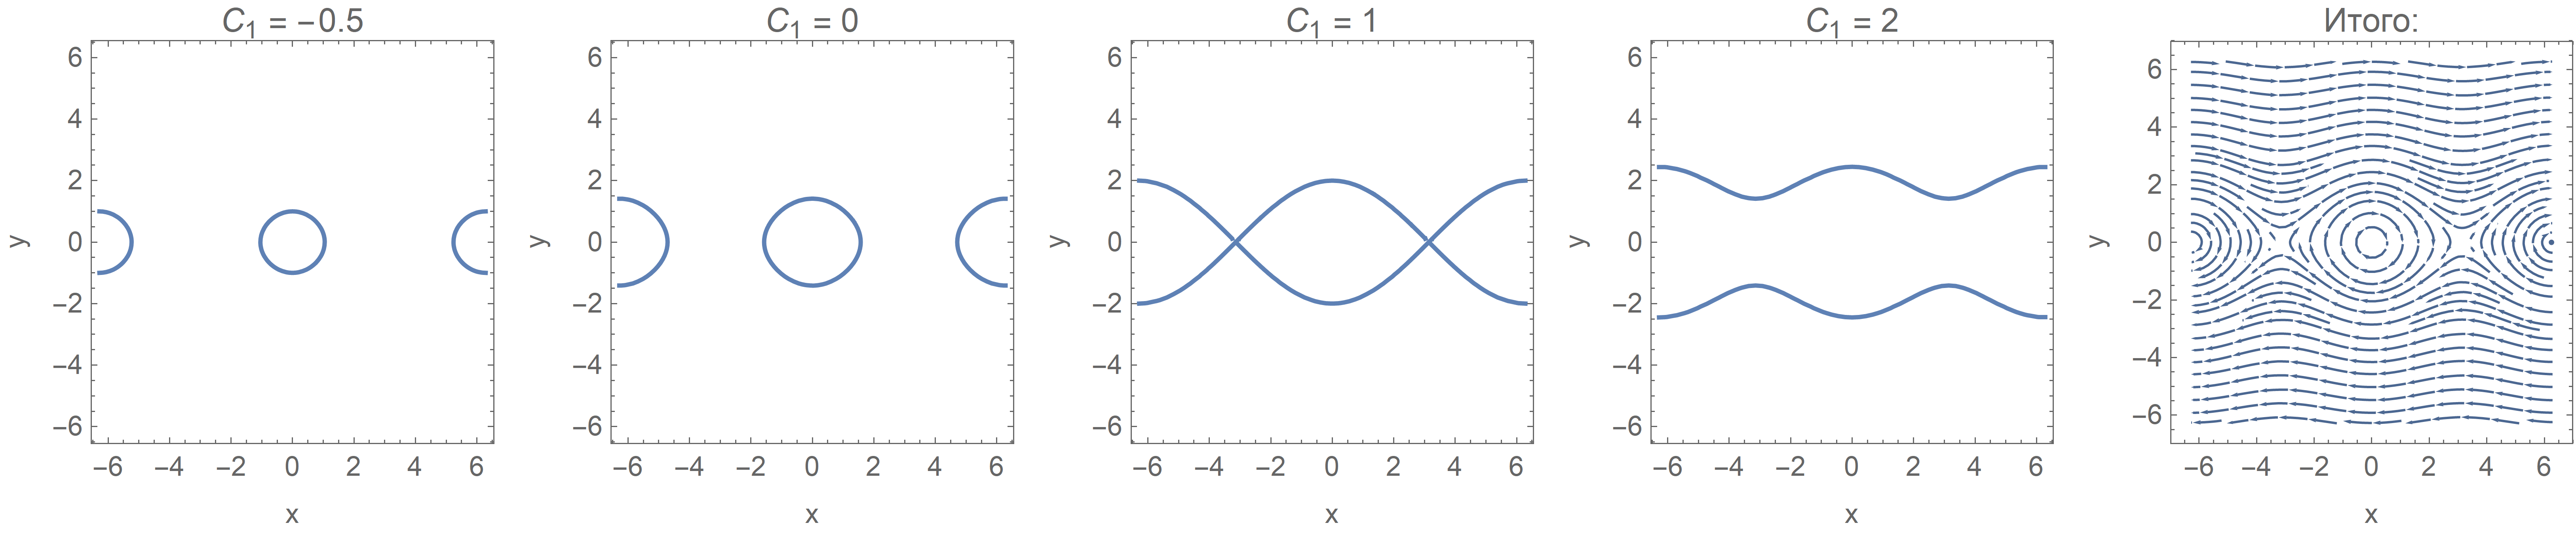
\includegraphics[width=1\linewidth]{T1a.png}}
\caption{Т1(a)}
\label{fig:Т1a}
\end{figure} \\
б) $\ddot x-x+x^2=0$ \\
Cделаем замену $\dot x = y$ тогда:
\begin{equation*}
    \begin{cases}
        \dot x=y\\
        \dot y = x-x^2
    \end{cases}
\end{equation*}
по правилу пропорции и обнуляя знаменатель:
\begin{gather*}
    \frac{\alpha dx + \beta dy}{\alpha y + \beta (x-x^2)}=dt \Rightarrow //\beta=y,\alpha=-(x-x^2)// \Rightarrow \\ 
    \Rightarrow -3x^2+2x^3+3y^2=C_1
\end{gather*}
Можно построить эту петельку: \ref{fig:Т1b}
\begin{figure}[h!]
\center{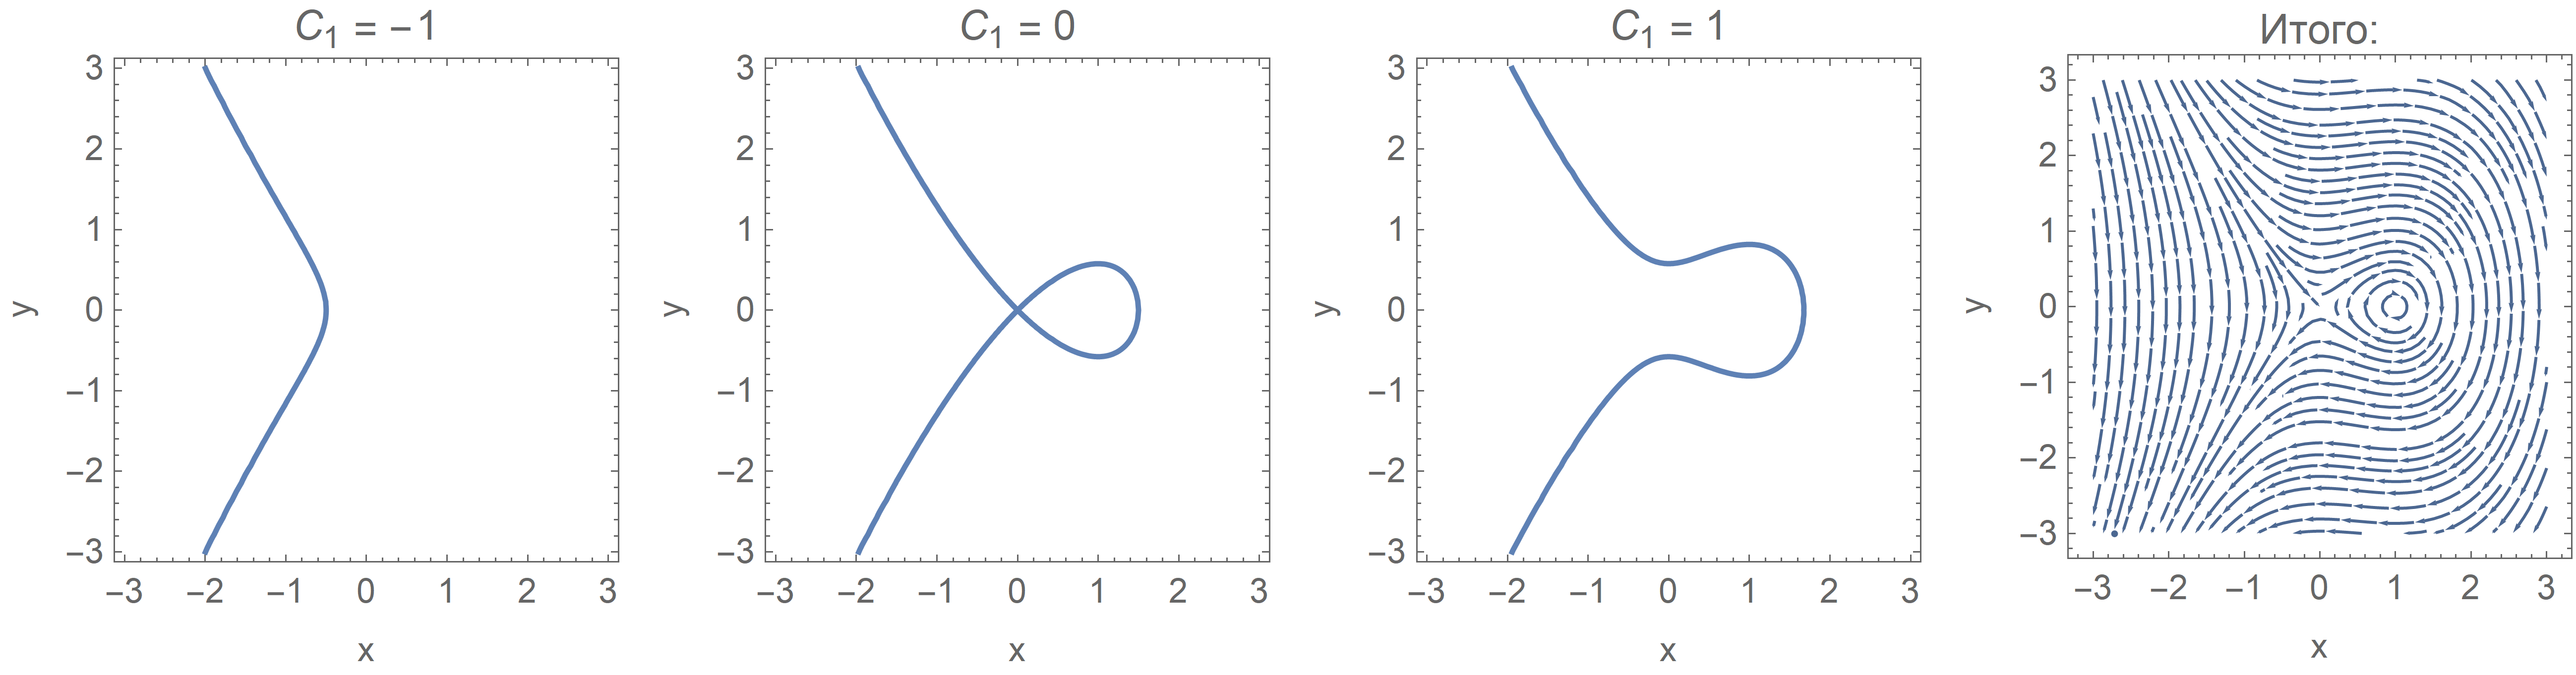
\includegraphics[width=1\linewidth]{T1b.png}}
\caption{Т1(б)}
\label{fig:Т1b}
\end{figure} \\

\subsection{C. \S16: 5}
Найдя первый интеграл, решить систему в указанной области
\begin{equation}\label{16.5}
    \begin{cases}
        \dot x = - \frac{x}{y},\\
        \dot y = \frac{y}{x}, (x>0,y>0).\\
    \end{cases}
\end{equation}
Поскольку $dx \frac{y}{x}+dy \frac{x}{y}=0$:
\begin{gather*}
    \frac{dy}{y^2}=-\frac{dx}{x^2}\\
    \frac{1}{y}=-\frac{1}{x}+C_1\\
    y = \frac{x}{C_1 x - 1}
\end{gather*}

Подставим $y$ в первое уравнение \ref{16.5}:
\begin{gather*}
    \dot x = 1-C_1 x\\
    \frac{dx}{1-C_1x}=dt\\
    x=\frac{C_2}{C_1}e^{-C_1t}+\frac{1}{C_1}
\end{gather*}
Подставим $x$ в $y$ и получаем ответ:\\
Ответ: $x=\frac{C_2}{C_1}e^{-C_1t} + \frac{1}{C_1}$, $y=  \frac{e^{C_1t}}{C_1 C_2} + \frac{1}{C_1} $
 \textcolor[rgb]{0.480469,0.566406,0.480469}{\textit{ответ не сходится с ответом в учебнике в силу разных обозначений $C_2$. Так-то ответ мой правильный (ответ учебника я в вольфраме не проверял)}}                                               

\subsection{C. \S16: 26}   
Найдя два независимых первых интеграла системы, решить систему в указанной области.
\begin{equation}\label{16.26}
    \begin{cases}
        \dot x = x^2,\\
        \dot y = 2x^3-xy-z,\\
        \dot z = xz - 2x^4, (x>0)
    \end{cases}
\end{equation}
Хмм, кажется что первое уравнение системы интегрируется. Ну раз так, проинтегрируем: $x=\frac{1}{C_1-t}$. Далее смотрим на оставшиеся 2 уравнения. Возьмём то в котором кроме $x$ не более 1 другой переменной. Т.е. третье. Подставив $x$ можем получить:
\begin{gather*}
    \dot z = \frac{z}{C_1-t} -2 \frac{1}{(C_1-t)^4}\\
    // \tau = C_1-t, \dot z = -\frac{dz}{d \tau}=-z'  // \\
    z'+\frac{z}{\tau}=2 \frac{1}{\tau^4}\\
    // \text{О, это же уравнение Эйлера, его мы умеем решать заменой } \tau=e^T, z'_\tau=z'_T e^{-T}// \\
    z'+z=2e^{-3T}\\
    //\text{находит общее, угадываем частное, благо тут оно очевидное и получаем ответ}// \\
    z(T)=C_2 e^{-T}-e^{-3T}=z(\tau)=\frac{C_2}{\tau}-\frac{1}{\tau^3}=z(t)=\frac{C_2}{C_1-t}-\frac{1}{(C_1-t)^3}
\end{gather*}
Теперь подставим $x(t)$ и $z(t)$ во второе уравнение системы \ref{16.26}:
\begin{gather*}
    \dot y = \frac{3}{(C_1-t)^3}-\frac{C_2}{(C_1-t)}-\frac{y}{C_1-t}\\
    //C_1-t=e^{T}, \dot y = y'_T e^{-T}//\\
    -y' e^{-T} = 3e^{-3T}-C_2 e^{-T}-y e^{-T}\\
    y'-y=C_2-3e^{-2T}\\
    y(T)=C_3 e^T-C_2+e^{-2 T}=y(t)=C_3(C_1-t)-C_2+\frac{1}{(C_1-t)^3}
\end{gather*}
И чтобы посмотреть на этот ужас скопанованно:\\
Ответ: $x(t)=\frac{1}{C_1-t}$,\\
        $y(t)=C_3(C_1-t)-C_2+\frac{1}{(C_1-t)^3}$,\\
        $z(t)=\frac{C_2}{C_1-t}-\frac{1}{(C_1-t)^3}$.



\section{II. Линейные однородные уравнения в частных производных первого порядка}
\subsection{C. \S17: 5}
\subsection{C. \S17: 16}
\subsection{C. \S17: 22}
\subsection{C. \S17: 79}
\subsection{C. \S17: 83}
\subsection{T2}

\section{III. Вариационное исчисление}
\subsection{C. \S19: 21}
\subsection{C. \S19: 45}
\subsection{C. \S19: 72}
\subsection{C. \S19: 105}
\subsection{T3}
\subsection{C. \S20.1: 9}
\subsection{C. \S20:}
\subsection{T4}
\subsection{C. \S20.2: 5}
\subsection{C. \S20.3: 2}
\subsection{C. \S21: 1}
\subsection{T5*}

\end{document}
